\documentclass[11pt]{article}
\usepackage[margin=1in]{geometry}
\usepackage{fontspec}
\usepackage{booktabs}
\usepackage{array}
\usepackage{float}
\usepackage{graphicx}
\usepackage{adjustbox}
\usepackage{amsmath}
\usepackage[font=small,labelfont=bf]{caption}
\usepackage{natbib}
\usepackage{xurl}
\usepackage[hidelinks]{hyperref}
\usepackage{setspace}
\setstretch{1.15}
\graphicspath{{../figs/}}
\newcommand{\nRecords}{1,868}
\newcommand{\nEligible}{359}
\newcommand{\nAnalysis}{343}
\newcommand{\nDem}{192}
\newcommand{\nRep}{106}
\newcommand{\nInd}{45}
\newcommand{\nDemFirst}{187}
\newcommand{\nRepFirst}{156}
\newcommand{\nCcesDem}{20,246}
\newcommand{\nCcesRep}{14,484}
\newcommand{\nGssDem}{699}
\newcommand{\nGssRep}{442}
\newcommand{\richOut}{36}
\newcommand{\richIn}{14}
\newcommand{\richTruth}{6.5}
\newcommand{\manRepOut}{93}
\newcommand{\manRepIn}{87}
\newcommand{\unionOut}{42}
\newcommand{\unionIn}{31}
\newcommand{\unionTruth}{9}
\newcommand{\atheistIn}{25}
\newcommand{\atheistTruth}{11}
\newcommand{\atheistGss}{8}
\newcommand{\blackOut}{25}
\newcommand{\blackIn}{18}
\newcommand{\blackTruth}{29}
\newcommand{\blackGss}{32}
\newcommand{\blackLr}{21}
\newcommand{\oldDemOut}{12}
\newcommand{\oldDemIn}{7}
\newcommand{\oldDemTruth}{43}
\newcommand{\oldRepOut}{31}
\newcommand{\oldRepIn}{25}
\newcommand{\oldRepTruth}{51}
\newcommand{\unemployedOut}{23}
\newcommand{\unemployedIn}{7}
\newcommand{\unemployedCces}{19}
\newcommand{\unemployedGss}{9}
\newcommand{\noCollegeOut}{34}
\newcommand{\noCollegeIn}{15}
\newcommand{\noCollegeTruth}{41}
\newcommand{\hitDemIn}{54}
\newcommand{\hitDemOut}{49}
\newcommand{\hitRepIn}{61}
\newcommand{\hitRepOut}{60}
\newcommand{\bestDem}{64}
\newcommand{\matchDem}{55}
\newcommand{\thetaIn}{-0.02}
\newcommand{\thetaOut}{0.31}
\newcommand{\thetaOutLo}{0.18}
\newcommand{\thetaOutHi}{0.42}
\newcommand{\thetaOutDouble}{1.24}
\newcommand{\thetaInNoRace}{0.44}
\newcommand{\thetaOutNoRace}{0.97}
\newcommand{\gap}{9.2}
\newcommand{\gapLo}{4.6}
\newcommand{\gapHi}{13.8}
\newcommand{\gapParty}{11.0}
\newcommand{\gapPartyLo}{6.7}
\newcommand{\gapPartyHi}{15.4}
\newcommand{\gapNoRace}{9.6}
\newcommand{\gapNoUnion}{8.9}
\newcommand{\gapGss}{5.0}
\newcommand{\gapGssLo}{1.1}
\newcommand{\gapGssHi}{8.8}
\newcommand{\gapCells}{9}
\newcommand{\gapCellsGss}{11}
\newcommand{\projAgeIn}{0.41}
\newcommand{\projAgeOut}{0.17}
\newcommand{\projSexIn}{0.19}
\newcommand{\projSexOut}{0.06}
\newcommand{\orderUnionFirst}{27}
\newcommand{\orderUnionSecond}{44}
\newcommand{\orderUnionHolm}{0.018}
\newcommand{\orderShareDemFirst}{52}
\newcommand{\orderShareDemSecond}{61}
\newcommand{\orderChisqP}{0.23}
\newcommand{\nOrderTests}{16}
\newcommand{\extN}{298}
\newcommand{\extMean}{2.32}
\newcommand{\extSd}{0.68}
\newcommand{\extStereo}{0.053}
\newcommand{\extStereoLo}{0.008}
\newcommand{\extStereoHi}{0.099}
\newcommand{\extRecall}{-0.41}
\newcommand{\extRecallLo}{-0.91}
\newcommand{\extRecallHi}{0.08}
\newcommand{\extStereoRange}{0.43}
\newcommand{\bootReps}{1,000}

\newcommand{\TableStyle}{\small\setlength{\tabcolsep}{5pt}\renewcommand{\arraystretch}{1.05}}

\title{Picturing the Other Party: What Partisans Guess about a Randomly Drawn Democrat and Republican}
\author{Douglas J. Ahler \and Gaurav Sood}
\date{}

\begin{document}
\maketitle

\begin{abstract}
\noindent We asked \nAnalysis{} Democrats, Republicans, and independents to guess the class, religion, race, sex, age, education, employment, and union membership of one randomly drawn Democrat and one randomly drawn Republican. A best guess about a single draw has a correct answer, the category most common in the party, and it requires no estimate of a percentage. Scored against the 2012 CCES and GSS, partisans picked that category less often than they could have, and they missed in a particular direction when guessing about the other party: they over-picked the category that sets that party apart from their own. In the cells where the most distinctive category is not the most common one, opposing partisans chose it \gap{} percentage points more often than co-partisans did (95\% CI \gapLo{} to \gapHi{}). Republicans imagined the Democrat as poor, unemployed, without college, and in a union more often than Democrats did; Democrats imagined the Republican as rich far more often than Republicans did. Both sides pictured the Republican as a man. Race is the exception: being Black is the trait most distinctive of Democrats, and both sides under-guessed it. Partisans who chose more of the other party's distinctive categories also placed that party further from the center.
\end{abstract}

\section{Introduction}

Partisans who guess the background of a randomly drawn member of the other party lean toward what sets that party apart. Asked about a random Republican, \richOut\% of Democrats guessed the person was rich; in the 2012 General Social Survey, \richTruth\% of Republicans call themselves upper class, and \richIn\% of Republicans in our sample guessed rich. Asked about a random Democrat, \unionOut\% of Republicans guessed the person belonged to a union, against \unionIn\% of Democrats and a population share near \unionTruth\%. Across the cells where the most distinctive category is not the most common one, opposing partisans chose the distinctive category \gap{} percentage points more often than co-partisans did.

The evidence comes from a 2013 survey that asked people to guess, one category at a time, the background of a Democrat and a Republican described as randomly drawn from a representative survey. That task differs from the usual measure of party stereotypes, which asks people what percentage of a party belongs to a group \citep{ahler2018parties, levendusky2016misperceptions}. Percentage estimates mix stereotyping with innumeracy and with ignorance of how common a group is in the population, and separating them requires additional experiments \citep{ahler2018parties}. A best guess about one draw avoids both problems. The answer that is most often right is simply the category most common in the party, and reporting it requires no arithmetic.

The guess task also gives a direct test of a model of stereotypes built on the representativeness heuristic \citep{kahneman1972subjective, bordalo2016stereotypes}. The model says people judge a group by the types that are more common in it than in a comparison group, so they overweight what is distinctive and underweight what is merely common. Applied to parties, it predicts that a Democrat asked to picture a Republican will reach for ``rich'' even though most Republicans are middle class, because Republicans are more likely than Democrats to be rich. Earlier work shows that party stereotypes are exaggerated \citep{ahler2018parties, rothschild2019pigeonholing}, that people picture engaged ideologues when they think of the other side \citep{druckman2022misestimating}, and that experimentally induced representativeness reasoning produces party stereotypes \citep{ahler2023typecast}. What has been missing is evidence on what people produce when simply asked to describe a typical partisan, measured against a population benchmark.

Three further results qualify the main one. The guesses are no more accurate than guessing in proportion to the true shares, so respondents do not reliably pick the most common category for either party. Both sides share some distortions, picturing the Republican as a man and the Democrat as young and nonreligious. And the strongest stereotype by the representativeness logic, that a Democrat is Black, shows up as an underestimate on both sides.

\section{Data and Design}

\subsection{The survey}

The survey ran on Amazon's Mechanical Turk in November 2013. Of \nRecords{} survey records, \nEligible{} belonged to respondents who passed a screen filling quotas for Democrats, Republicans, and independents, and \nAnalysis{} of them reached the guessing task: \nDem{} Democrats, \nRep{} Republicans, and \nInd{} independents, counting leaners as partisans. Every eligible respondent has a distinct worker ID, so no further de-duplication was needed.

Respondents read that the researchers had ``recently conducted a representative survey of Americans'' and had ``randomly paired you with two respondents from that survey (one Democrat and one Republican).'' They then guessed eight characteristics of each: class (poor, middle class, rich), religion (born-again or evangelical Christian, other Protestant, Catholic, Jewish, atheist or agnostic, something else), race (White, Black, Asian), sex, age (18--35, 36--50, 50+), whether the person had gone to college, whether the person was employed, and union membership. The respondent numbers shown were random integers; the guesses are about a random draw, not about a real record, and we score them against population shares. Whether the Democrat or the Republican came first was randomized (\nDemFirst{} saw the Democrat first, \nRepFirst{} the Republican). The same survey asked respondents to name leaders who come to mind for each party and to place both parties on a seven-point liberal--conservative scale. The full instrument is in the replication materials.

\subsection{Population benchmarks}

We take population shares from the 2012 Cooperative Congressional Election Study \citep{cces2012}, which has \nCcesDem{} Democrats and \nCcesRep{} Republicans, and from the 2012 General Social Survey \citep{gss2012}, which has \nGssDem{} and \nGssRep{}. Partisans are self-identified Democrats and Republicans without leaners; counting leaners changes little (Appendix Table~\ref{tab:choice-sens}). Both surveys are weighted. The CCES supplies every attribute except class, which it does not ask about; class comes from the GSS question on subjective social class, with lower class coded poor, working and middle class coded middle class, and upper class coded rich.

Several answer options do not map exactly onto survey questions, and we chose the mapping before estimating anything. ``College educated'' is set against ``never went to college,'' so people with some college count as college educated; a stricter coding that drops them is a sensitivity check. ``Unemployed'' is measured among people in the labor force; counting everyone not working as unemployed is a second check. The race question offered only White, Black, and Asian, so shares are computed among people in those three groups. Appendix Table~\ref{tab:benchmarks} gives every share from both sources. They agree on the most common category for every attribute except the religion of Democrats, where the CCES puts ``something else'' first (largely people with no particular religion) and the GSS puts born-again Christians first.

\subsection{What a guess can be compared with}

Each guess is scored three ways. The first is whether it names the category most common in the target's party. The second is the chance that the guess would match a randomly drawn partisan, which equals the population share of the category guessed. Always guessing the most common category maximizes this chance; guessing each category in proportion to its population share yields the sum of squared shares, a natural baseline for someone who knows the distribution but samples from it.

The third score concerns how distinctive the guessed category is. For each category we compute the likelihood ratio: its share in the target's party divided by its share in the other party. Being Black, for example, is \blackLr{} times as common among Democrats as among Republicans in the CCES. The representativeness model predicts that guesses lean toward categories with high likelihood ratios even when those categories are rare.

\section{How Accurate Are the Guesses?}

Respondents chose the most common category on roughly three of every five attributes, well short of what consistently naming it would achieve (Table~\ref{tab:accuracy}). Scored by the chance of matching a random draw, Democrats' guesses about a Democrat were right \hitDemIn\% of the time and Republicans' guesses about a Democrat \hitDemOut\%, against \bestDem\% for always naming the most common category and \matchDem\% for guessing in proportion to the shares. Guesses about a Republican were more accurate, \hitRepIn\% for Republicans and \hitRepOut\% for Democrats, mainly because Republicans are more homogeneous: more of them are White, employed, and not in a union. On no comparison do guesses beat proportional guessing by much, and Republicans' guesses about a Democrat fall below it.

\begin{table}[htbp]
\centering\TableStyle
\caption{Accuracy of guesses about a randomly drawn partisan, averaged over eight attributes.}
\label{tab:accuracy}
\adjustbox{max width=\linewidth}{\begin{tabular}{llccccr}
\toprule
Guesses about & Guessers & Chose modal category (\%) & Correct by chance (\%) & Proportional guessing (\%) & Always the mode (\%) & $n$ \\
\midrule
Democrat & Co-partisans & 59 [57, 61] & 54 [53, 55] & 55 & 64 & 192 \\
Democrat & Opposing partisans & 53 [49, 56] & 49 [47, 51] & 55 & 64 & 106 \\
Republican & Co-partisans & 64 [61, 66] & 61 [60, 63] & 63 & 71 & 106 \\
Republican & Opposing partisans & 63 [61, 65] & 60 [59, 61] & 63 & 71 & 192 \\
\bottomrule
\end{tabular}
}
\begin{minipage}{\linewidth}\footnotesize\vspace{4pt}
\emph{Note}: ``Chose modal category'' is the share of guesses naming the category most common in the target's party. ``Correct by chance'' is the probability that a guess matches a randomly drawn partisan, the population share of the category guessed. ``Proportional guessing'' is the accuracy of guessing each category in proportion to its population share, and ``Always the mode'' the accuracy of always naming the most common category. Each respondent's eight guesses about a target are averaged before averaging across respondents. 95\% intervals from \bootReps{} respondent bootstrap draws. Benchmarks: CCES 2012, with class from the GSS 2012.
\end{minipage}
\end{table}

Figure~\ref{fig:guesses} shows where the guesses go wrong. Some errors are shared by both sides and have nothing to do with which party is being judged. Few respondents guessed that the Democrat was 50 or older (\oldDemIn\% of Democrats, \oldDemOut\% of Republicans), though \oldDemTruth\% of Democrats are; respondents did better for the Republican, at \oldRepIn\% and \oldRepOut\%, against \oldRepTruth\%. Both sides pictured the Republican as a man (\manRepIn\% of Republicans, \manRepOut\% of Democrats), though roughly half of Republicans are women. Both sides chose ``atheist or agnostic'' for the Democrat \atheistIn\% of the time, against \atheistTruth\% in the CCES and \atheistGss\% in the GSS.

\begin{figure}[htbp]
\centering
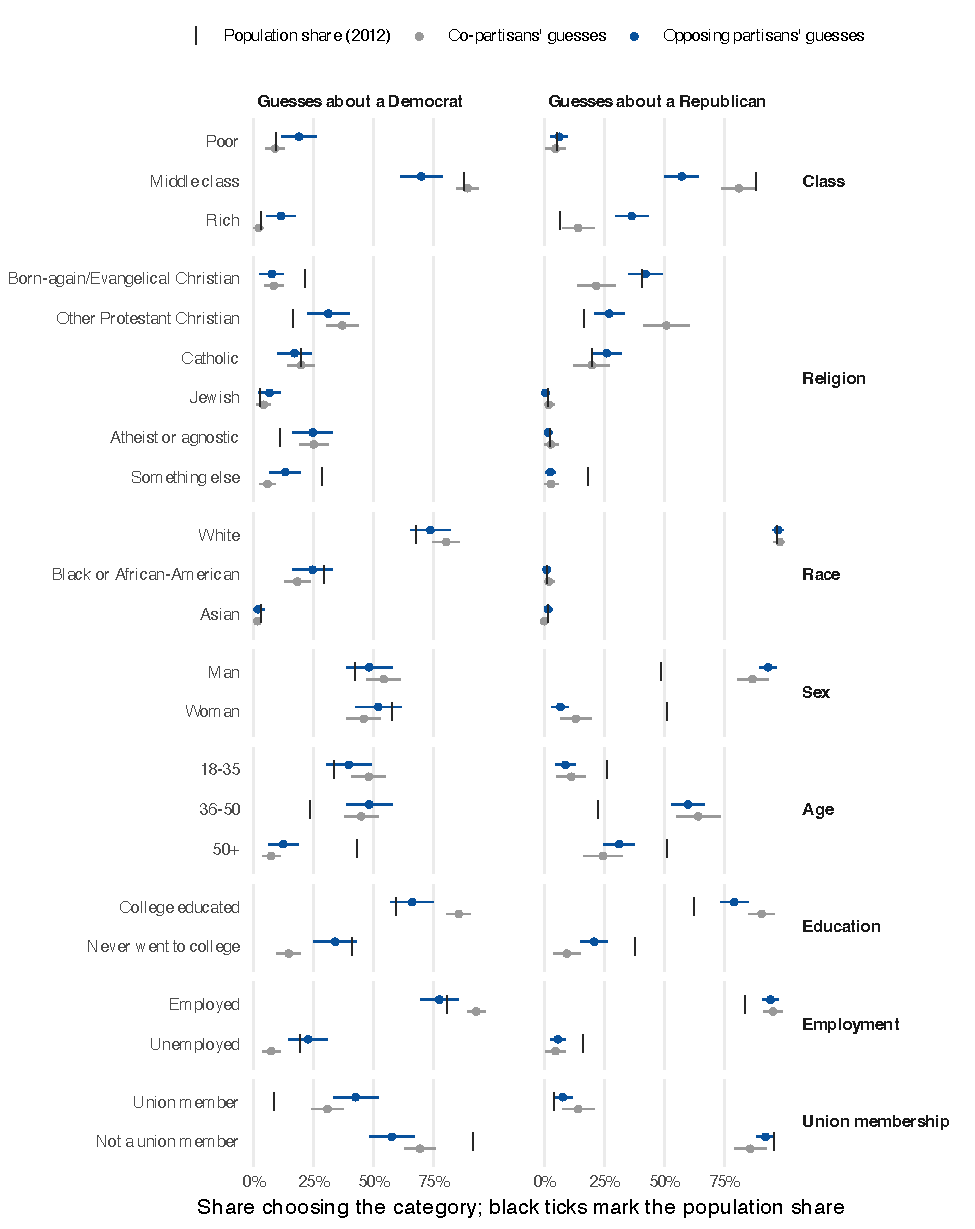
\includegraphics[width=\linewidth,height=0.82\textheight,keepaspectratio]{guesses_vs_truth.pdf}
\caption{Guesses about a randomly drawn Democrat (left) and Republican (right), by whether the guesser shares the target's party. Dots are the share of respondents choosing each category, with 95\% intervals; black ticks are the population share among self-identified partisans in the CCES 2012 (class: GSS 2012). Co-partisans: \nDem{} Democrats guessing about the Democrat and \nRep{} Republicans about the Republican; opposing partisans the reverse. Independents are omitted.}
\label{fig:guesses}
\end{figure}

\section{Opposing Partisans Lean toward What Is Distinctive}

The errors that differ by side follow the likelihood ratio. Republicans guessed that the Democrat had never gone to college \noCollegeOut\% of the time and was unemployed \unemployedOut\% of the time; Democrats guessed \noCollegeIn\% and \unemployedIn\%. Democrats guessed the Republican was rich \richOut\% of the time; Republicans guessed \richIn\%. For education, and for unemployment as the CCES measures it, the opposing side's guess is the closer one: \noCollegeTruth\% of Democrats never went to college, and the share unemployed is \unemployedCces\% in the CCES and \unemployedGss\% in the GSS. So co-partisans under-guess their own party's less flattering distinctive traits at least as much as opposing partisans over-guess them. Where the distinctive trait is rare, as with rich Republicans and union Democrats, the opposing side's guesses are much further from the population share.

Figure~\ref{fig:gap} isolates the comparison. It takes the cells where the most distinctive category is not the most common one, \gapCells{} with the primary benchmarks, and compares how often opposing partisans and co-partisans chose the distinctive category. Pooling the cells, with cell fixed effects and standard errors clustered by respondent, opposing partisans chose it \gap{} percentage points more often (95\% CI \gapLo{} to \gapHi{}). Adjusting for the respondent's own party, so that a general tendency of Democrats or Republicans to choose rarer categories cannot masquerade as an out-party effect, the gap is \gapParty{} points (\gapPartyLo{} to \gapPartyHi). Dropping race gives \gapNoRace{} points. With the GSS benchmarks for every attribute, \gapCellsGss{} cells qualify and the gap is \gapGss{} points (\gapGssLo{} to \gapGssHi); the two added cells have likelihood ratios close to one.

\begin{figure}[htbp]
\centering
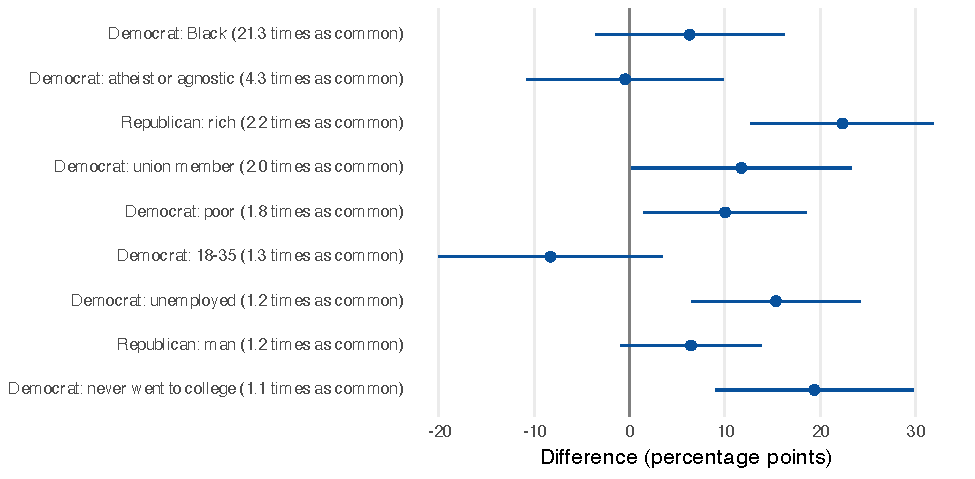
\includegraphics[width=\linewidth]{diagnostic_gap.pdf}
\caption{Opposing minus co-partisan share choosing the category most distinctive of the target's party, in the cells where that category is not the most common one. The ratio in parentheses is how many times as common the category is in the target's party as in the other party (CCES 2012; class: GSS 2012). Lines are 95\% intervals from heteroskedasticity-robust (HC2) standard errors; each respondent answers each cell once.}
\label{fig:gap}
\end{figure}

The exception is race. Being Black is by far the most distinctive trait of Democrats, yet both sides under-guessed it: \blackIn\% of Democrats and \blackOut\% of Republicans guessed the Democrat was Black, against \blackTruth\% in the CCES and \blackGss\% in the GSS. The representativeness model does not predict this, and it contrasts with percentage estimates, in which partisans overstate the share of Democrats who are Black \citep{ahler2018parties}. One possibility is that respondents avoided a single-person answer that could look like racial stereotyping.

A conditional logit model summarizes all categories at once. Each guess is a choice among the offered categories, and the probability of choosing a category is proportional to its population share raised to a power $\gamma$ times its likelihood ratio raised to a power $\theta$. Guessing in proportion to the shares corresponds to $\gamma=1$ and $\theta=0$; always naming the most common category corresponds to a very large $\gamma$; the representativeness model implies $\theta>0$. Table~\ref{tab:choice} reports the estimates. For opposing partisans $\theta$ is \thetaOut{} (\thetaOutLo{} to \thetaOutHi), so doubling a category's likelihood ratio, holding its population share fixed, multiplies the odds of choosing it by \thetaOutDouble. For co-partisans it is \thetaIn. Both $\gamma$ estimates are below one: guesses are spread more evenly across categories than the population is.

\begin{table}[htbp]
\centering\TableStyle
\caption{Conditional logit estimates of how guesses respond to a category's population share and its likelihood ratio.}
\label{tab:choice}
\adjustbox{max width=\linewidth}{\begin{tabular}{lccr}
\toprule
Guessers & Weight on population share & Weight on diagnosticity & Respondents \\
\midrule
Co-partisans & 0.81 [0.74, 0.87] & -0.02 [-0.10, 0.05] & 298 \\
Opposing partisans & 0.65 [0.58, 0.72] & 0.31 [0.18, 0.42] & 298 \\
Independents & 0.68 [0.57, 0.80] & 0.05 [-0.10, 0.19] &  45 \\
\bottomrule
\end{tabular}
}
\begin{minipage}{\linewidth}\footnotesize\vspace{4pt}
\emph{Note}: Each guess is a choice among the offered categories, with probability proportional to $\text{share}^{\gamma}\,\text{LR}^{\theta}$. The weight on population share is $\gamma$; the weight on diagnosticity, $\theta$, multiplies the log of the likelihood ratio (share in the target's party over share in the other party). 95\% intervals from \bootReps{} bootstrap draws that resample respondents and redraw benchmark shares from their sampling distribution.
\end{minipage}
\end{table}

The model fits a single $\theta$ across attributes whose likelihood ratios range from about one to more than twenty, so one attribute can move it. Race does: without race, $\theta$ is \thetaInNoRace{} for co-partisans and \thetaOutNoRace{} for opposing partisans (Appendix Table~\ref{tab:choice-sens}). The finding that survives every specification is the ordering, opposing partisans above co-partisans, not the co-partisan estimate of zero. We therefore lead with the cell-by-cell comparison rather than with $\theta$ itself.

A competing explanation is projection: people may answer with their own characteristics, especially when picturing their own party. Comparing respondents who differ on a characteristic, co-partisans were \projAgeIn{} more likely (as a proportion) to give the Democrat or Republican their own age group and \projSexIn{} more likely to give their own sex; for opposing partisans the figures were \projAgeOut{} and \projSexOut{} (Appendix Table~\ref{tab:projection}). Projection thus shapes guesses about one's own party more than about the other. It cannot produce the out-party pattern in Figure~\ref{fig:gap}, which concerns traits such as class, employment, and union membership that the projection estimates do not cover and that the gap compares within the same cell.

\section{Question Order}

Asking about the Democrat or the Republican first made no detectable difference to the number of distinctive categories chosen (Table~\ref{tab:order}). Of the \nOrderTests{} attribute-level comparisons, one survives a Holm correction: respondents asked about the Democrat second guessed union membership \orderUnionSecond\% of the time, against \orderUnionFirst\% when the Democrat came first (adjusted $p=\orderUnionHolm$). That item contains a programming error. In the block that asked about the Democrat first, the union question displayed the Republican's respondent number instead of the Democrat's. The order difference on that item therefore may reflect the error rather than question order, and removing the item changes the main comparison little (\gapNoUnion{} points). The proportion of Democrats differed somewhat between the two orders (\orderShareDemFirst\% and \orderShareDemSecond\%; $\chi^2$ test $p=\orderChisqP$).

\begin{table}[htbp]
\centering\TableStyle
\caption{Effect of being asked about a party second rather than first.}
\label{tab:order}
\adjustbox{max width=\linewidth}{\begin{tabular}{llcc}
\toprule
Outcome & Guesses about & Asked first & Difference if asked second \\
\midrule
Most diagnostic categories chosen (of 8) & Democrat & 2.26 & -0.13 [-0.47, 0.21] \\
Most diagnostic categories chosen (of 8) & Republican & 5.46 & 0.02 [-0.24, 0.27] \\
Chose union member (proportion) & Democrat & 0.27 & 0.17 [0.07, 0.27] \\
Chose union member (proportion) & Republican & 0.07 & 0.07 [0.00, 0.13] \\
\bottomrule
\end{tabular}
}
\begin{minipage}{\linewidth}\footnotesize\vspace{4pt}
\emph{Note}: Order was randomized. ``Most diagnostic categories chosen'' counts, out of eight attributes, the guesses naming the category with the highest likelihood ratio for the target's party. 95\% intervals from HC2 standard errors; $n=\nAnalysis$ respondents. In the Democrat-first block, the union question about the Democrat displayed the Republican's respondent number.
\end{minipage}
\end{table}

\section{Stereotypes and the Perceived Extremity of the Other Party}

If stereotypes feed the sense that the other party is extreme, partisans who picture its distinctive types should also place it further from the center. They do, modestly. Among \extN{} partisans, the other party's distance from the midpoint of the seven-point scale averages \extMean{} (standard deviation \extSd). Each additional distinctive category chosen for the other party, out of eight, goes with a placement \extStereo{} points further out (95\% CI \extStereoLo{} to \extStereoHi), adjusting for strength of partisanship and party (Table~\ref{tab:extremity}). Across the full range of eight, that is \extStereoRange{} points.

The proposal that motivated the survey had a second source in mind: partisans who think of more extreme leaders should see the other party as more extreme. The survey can check this too, using the ideological scores of the opposing-party leaders each respondent named first. The estimate runs the other way, \extRecall{} (\extRecallLo{} to \extRecallHi). Both associations are cross-sectional; they are consistent with stereotypes shaping perceived extremity, with perceived extremity shaping stereotypes, or with both responding to political engagement.

\begin{table}[htbp]
\centering\TableStyle
\caption{Perceived extremity of the other party, regressed on stereotyped guesses and the leaders recalled.}
\label{tab:extremity}
\adjustbox{max width=\linewidth}{\begin{tabular}{p{6.2cm}ccc}
\toprule
  & (1) & (2) & (3) \\
\midrule
Most diagnostic categories chosen for the opposing party (0--8) & 0.05 [0.01, 0.10] &  & 0.05 [0.01, 0.10] \\
Mean CF-score of opposing leaders recalled (toward their pole) &  & -0.40 [-0.91, 0.11] & -0.41 [-0.91, 0.08] \\
Strength of partisanship (1--3) & 0.12 [0.02, 0.21] & 0.13 [0.03, 0.23] & 0.12 [0.03, 0.22] \\
Republican respondent & 0.07 [-0.14, 0.28] & -0.07 [-0.24, 0.10] & 0.09 [-0.12, 0.30] \\
Constant & 1.80 [1.45, 2.15] & 2.46 [1.91, 3.00] & 2.18 [1.58, 2.77] \\
Respondents & 298 & 293 & 293 \\
\bottomrule
\end{tabular}
}
\begin{minipage}{\linewidth}\footnotesize\vspace{4pt}
\emph{Note}: Outcome is the absolute distance of the respondent's placement of the other party from 4 on a 1--7 liberal--conservative scale. Recalled leaders are scored with static CF-scores, signed so that positive values point toward the leader's own party's pole, averaged over up to three free-recall names; respondents with no scored name drop from columns 2 and 3. OLS with HC2 95\% intervals. Democratic and Republican respondents only.
\end{minipage}
\end{table}

\section{Discussion}

Partisans asked for a best guess about a random member of the other party reach for what makes that party different. The gap is moderate, \gap{} percentage points in the cells where it can be measured, and it sits beside larger errors that both sides share. The guess task removes two explanations that complicate percentage-based measures: no numeracy is needed, and the right answer does not depend on knowing how large a group is in the population, only on which category is most common in the party.

Three features of the study limit what it shows. The respondents were Mechanical Turk workers in 2013, not a probability sample, and the comparisons are among them. The guesses were not incentivized, so some may be expressive, although paying for accuracy left percentage estimates of party composition unchanged in earlier work \citep{ahler2018parties}. And the benchmarks rest on mappings between answer options and survey questions, most consequentially for class and for the religion of Democrats, where the two surveys disagree about the most common category. The main comparison holds under each alternative we examined, but the level of accuracy in Table~\ref{tab:accuracy} depends on them.

The race result deserves a direct test. A design that varies whether the guess is private or attributable would show whether the under-guessing of Black Democrats is a reporting choice or a belief.

\bibliographystyle{apsr}
\bibliography{references}

\clearpage
\appendix
\renewcommand{\thetable}{A\arabic{table}}
\setcounter{table}{0}
\section{Appendix}

\begin{table}[H]
\centering\TableStyle
\caption{Population shares by party, 2012 (percent).}
\label{tab:benchmarks}
\adjustbox{max width=\linewidth, max totalheight=0.85\textheight}{\begin{tabular}{lcccc}
\toprule
Category & CCES Dem. & GSS Dem. & CCES Rep. & GSS Rep. \\
\midrule
\multicolumn{5}{l}{\emph{Class}} \\
Poor & 18.5 & 9.5 & 11.8 & 5.3 \\
Middle class & 80.5 & 87.5 & 87.1 & 88.1 \\
Rich & 1.0 & 3.0 & 1.1 & 6.5 \\
\addlinespace
\multicolumn{5}{l}{\emph{Religion}} \\
Born-again/Evangelical Christian & 21.4 & 31.0 & 40.7 & 41.8 \\
Other Protestant Christian & 16.3 & 17.6 & 16.5 & 24.5 \\
Catholic & 19.9 & 25.4 & 20.2 & 21.7 \\
Jewish & 2.7 & 2.2 & 1.5 & 1.5 \\
Atheist or agnostic & 11.1 & 8.0 & 2.6 & 2.9 \\
Something else & 28.6 & 15.9 & 18.5 & 7.6 \\
\addlinespace
\multicolumn{5}{l}{\emph{Race}} \\
White & 67.6 & 63.9 & 96.9 & 94.1 \\
Black or African-American & 29.2 & 32.0 & 1.4 & 1.2 \\
Asian & 3.2 & 4.1 & 1.7 & 4.7 \\
\addlinespace
\multicolumn{5}{l}{\emph{Sex}} \\
Man & 42.2 & 40.2 & 48.7 & 47.1 \\
Woman & 57.8 & 59.8 & 51.3 & 52.9 \\
\addlinespace
\multicolumn{5}{l}{\emph{Age}} \\
18-35 & 33.5 & 30.6 & 26.3 & 27.7 \\
36-50 & 23.4 & 24.8 & 22.3 & 26.1 \\
50+ & 43.1 & 44.6 & 51.4 & 46.2 \\
\addlinespace
\multicolumn{5}{l}{\emph{Education}} \\
College educated & 59.2 & 61.1 & 62.2 & 66.6 \\
Never went to college & 40.8 & 38.9 & 37.8 & 33.4 \\
\addlinespace
\multicolumn{5}{l}{\emph{Employment}} \\
Employed & 80.7 & 90.6 & 83.8 & 95.4 \\
Unemployed & 19.3 & 9.4 & 16.2 & 4.6 \\
\addlinespace
\multicolumn{5}{l}{\emph{Union membership}} \\
Union member & 8.6 & 12.1 & 4.2 & 7.1 \\
Not a union member & 91.4 & 87.9 & 95.8 & 92.9 \\
\bottomrule
\end{tabular}
}
\begin{minipage}{\linewidth}\footnotesize\vspace{4pt}
\emph{Note}: Weighted shares among self-identified Democrats and Republicans. CCES class is family income (under \$20,000 poor, \$250,000 or more rich); the analysis uses GSS subjective class instead. GSS religion uses the belief-in-God item to separate atheists and agnostics from others with no religion; CCES religion uses the Pew items. College educated: any college. Unemployed: share of the labor force. Race: shares among White, Black, and Asian respondents.
\end{minipage}
\end{table}

\begin{table}[H]
\centering\TableStyle
\caption{Weight on diagnosticity ($\theta$) under alternative benchmarks and samples.}
\label{tab:choice-sens}
\begin{tabular}{lcc}
\toprule
Specification & Co-partisans & Opposing partisans \\
\midrule
Primary benchmarks & -0.02 (0.03) & 0.31 (0.06) \\
GSS for every attribute & -0.09 (0.04) & 0.24 (0.06) \\
Leaners counted as partisans & 0.04 (0.04) & 0.38 (0.06) \\
College = four-year degree & -0.02 (0.03) & 0.31 (0.06) \\
Unemployed = everyone not working & -0.02 (0.03) & 0.31 (0.05) \\
Race omitted & 0.44 (0.08) & 0.97 (0.09) \\
Union membership omitted & -0.04 (0.04) & 0.26 (0.06) \\
Democratic union item omitted & -0.06 (0.04) & 0.26 (0.06) \\
\bottomrule
\end{tabular}

\begin{minipage}{\linewidth}\footnotesize\vspace{4pt}
\emph{Note}: Conditional logit estimates as in Table~\ref{tab:choice}, standard errors clustered by respondent in parentheses.
\end{minipage}
\end{table}

\begin{table}[H]
\centering\TableStyle
\caption{Projection: difference in the probability of guessing a category between respondents who belong to it and those who do not.}
\label{tab:projection}
\begin{tabular}{llcr}
\toprule
Characteristic & Guessers & Difference (proportion) & $n$ \\
\midrule
Race & Co-partisans & 0.18 [0.01, 0.34] & 284 \\
Race & Opposing partisans & -0.03 [-0.12, 0.06] & 284 \\
Sex & Co-partisans & 0.19 [0.09, 0.30] & 298 \\
Sex & Opposing partisans & 0.06 [-0.04, 0.15] & 298 \\
Age & Co-partisans & 0.41 [0.32, 0.49] & 179 \\
Age & Opposing partisans & 0.17 [0.07, 0.27] & 179 \\
Education & Co-partisans & 0.20 [0.03, 0.37] & 298 \\
Education & Opposing partisans & 0.09 [-0.09, 0.26] & 298 \\
\bottomrule
\end{tabular}

\begin{minipage}{\linewidth}\footnotesize\vspace{4pt}
\emph{Note}: Linear probability models over respondent-by-category rows with category fixed effects; CR2 95\% intervals clustered by respondent. Own age was asked as 18--29, 30--49, or 50+, so only the 18--29 and 50+ groups are compared. Own education: high school only versus any college.
\end{minipage}
\end{table}

\end{document}
